%% Overleaf: Compiler = pdfLaTeX. TeX Live (any recent).
%% Run: pdflatex -> bibtex -> pdflatex -> pdflatex
%% IEEEtran is built into Overleaf. Figures sit in ./figures/
\documentclass[journal]{IEEEtran}

\usepackage[T1]{fontenc}
\usepackage{lmodern}
\usepackage{cite}
\usepackage{amsmath,amssymb,amsfonts}
\usepackage{graphicx}
\usepackage{booktabs}
\usepackage{tabularx}
\usepackage{stfloats}
\usepackage[caption=false,font=footnotesize]{subfig}
\usepackage{url}
\usepackage{algorithm}
\usepackage{algpseudocode}
\usepackage{hyperref}
\hypersetup{hidelinks,colorlinks=false}

\graphicspath{{figures/}{../figures/imu_gated_evs_hold/}}

\DeclareRobustCommand{\norm}[1]{\lVert #1 \rVert}

\begin{document}

\title{Zero-Velocity Detection for Holding Event-to-Video
Reconstructions on a Pure EVS Camera}

\author{Vyapak~Bansal%
\thanks{V. Bansal is with the Intelligent Navigation and Mapping Laboratory
(INML), Schulich School of Engineering, University of Calgary, Calgary, AB,
Canada (e-mail: vyapakbansal@gmail.com). This work was supervised by
Dr.~Hongzhou Yang.}}

\markboth{IEEE Transactions on Robotics (draft)}%
{Bansal: Zero-Velocity Detection for Holding Event-to-Video Reconstructions}

\maketitle

\begin{abstract}
A pure event vision sensor (EVS), such as the Lucid Triton2, has no concurrent
grayscale output, so there is no fallback image when a scene stops changing.
Recurrent event-to-video (E2V) networks like FireNet hold scene appearance in a
hidden state that every new window of events overwrites. When the camera stops,
the event rate collapses, the network is fed near-empty voxels anyway, and the
reconstruction fades within one to two seconds, taking any downstream feature
tracker or preview down with it. We treat this as a zero-velocity detection
(ZVD) problem, the still/moving test long used in inertial navigation, rather
than as a reconstruction-quality problem. Skog, Handel, Nilsson, and Rantakokko
showed that an angular-rate energy (ARE) detector using only the gyroscope beats
accelerometer-only tests, and that their fused detector (SHOE) improves on ARE
only marginally. We take from that result a narrow claim: a MEMS gyroscope is
sufficient to decide that a sensor is stationary, not how it is moving.
FireNet's ConvGRU state is then gated the way an INS error state is gated under
ZUPT: shut when still, open when moving.

We implement two holds in a CUDA/TensorRT pipeline (libeventgate). Empty-window
HOLD re-emits the last reconstruction when a 10\,ms window has zero events. An
ARE-style gate declares STATIC when \(\norm{\boldsymbol{\omega}} < \delta\) and, in
the released pipeline, latches a recent high-quality frame rather than
continuing to run FireNet on residual noise. On a 168\,s indoor Triton2
recording (Sony IMX637, \(640\times 512\), \(1.107\times 10^{9}\) events) with a
software-aligned MEMS IMU, both mechanisms are measured on the same bag.
Empty-window HOLD reuses one FireNet frame for 2.00\,s after the last event,
with the ORB count frozen at 1634. A freeze-hidden-state ablation of the ARE
gate at \(\delta = 0.08\)\,rad/s leaves MOVING windows essentially unchanged
(mean ORB 977 gated vs.\ 980 ungated) while STATIC windows drop sharply (mean
ORB 292 vs.\ 914, median 238 vs.\ 885): the gate is selectively suppressing the
exact windows it should, without disturbing motion. That ablation still runs
FireNet on sparse voxels while discarding its state update, so the emitted image
itself continues to fade; the released default instead skips inference after
1\,s of confirmed STATIC and re-emits a recent high-event-count frame from a
rolling buffer. That latch is measured on the same bag in
Section~\ref{sec:latch-results}: MOVING stays close to ungated, and long STATIC
bouts lock to identical canvases rather than continuing to fade. A shared-gate
specification lets a stereo EVS pair use one still/moving decision instead of
two independent ones. Gyro-only ZVD cannot see translation that produces no
rotation; we treat this as a known limit of the detector on an unconstrained
mount, not a challenge to Skog's original gait results, and outline the direct
extension (SHOE, a higher-rate IMU) that addresses it.
\end{abstract}

\begin{IEEEkeywords}
Event camera, event-to-video reconstruction, FireNet, zero-velocity detection,
MEMS IMU, angular-rate energy, ConvGRU, stereo event cameras.
\end{IEEEkeywords}

\section{Introduction}
\IEEEPARstart{A}{conventional} camera integrates light over a fixed exposure and
outputs a dense frame at a fixed rate whether or not the scene moves. An event
camera reports only change: each pixel fires independently when its
log-intensity crosses a threshold, producing tuples \((x,y,t,p)\) at microsecond
resolution \cite{gallego2022}. High dynamic range, low latency, and negligible
motion blur are why these sensors have found traction in robotics and driving
\cite{gallego2022,zhou2021,gehrig2020}. The same asynchronous design means a
static scene produces almost no data at all. The Lucid Triton2 (Sony IMX637)
used in this work is a pure EVS device \cite{lucid_triton2}: unlike a DAVIS
sensor, it does not additionally output a synchronized grayscale frame
\cite{gallego2022}. Any stage downstream that needs an intensity image has to
reconstruct one from events alone, with nothing to fall back on.

E2VID \cite{rebecq2021} and the much smaller FireNet \cite{scheerlinck2020} both
map a voxel grid of recent events to an image while carrying a hidden state
\(h_t\) across time, and FireNet in particular depends on that recurrence: its
receptive field is too small to build a scene from a single window in isolation
\cite{scheerlinck2020}. This is exactly what breaks at a stop. Relative motion
goes to zero, pixels stop firing except for noise and hot pixels, the near-empty
voxel is fed to the network anyway, \(h_t\) is overwritten, and the
reconstruction fades to gray grain within roughly one to two seconds
\cite{scheerlinck2020}. ORB or FAST tracking, a live preview, or a detector then
loses input that was never actually gone, only forgotten by the network
responsible for holding it.

A frame camera has no such failure mode: pointed at a still scene, it keeps
producing the same picture, because capture never depended on motion in the
first place. What pure EVS needs is an external signal that the sensor is not
moving, so the last valid reconstruction can be held instead of allowed to
decay. Framed this way, the problem is not new. It is the same binary decision
inertial navigation has studied for two decades as zero-velocity detection.

Skog \textit{et al.} \cite{skog2010tbe} placed the classical ZVD detectors
(acceleration moving variance, acceleration magnitude, and angular-rate energy)
inside one generalized likelihood-ratio framework and derived a fused detector,
SHOE, from all three priors. On foot-mounted gait data, ARE alone outperformed
both accelerometer tests, and SHOE improved on ARE only marginally
\cite{skog2010tbe,skog2010ipin}. A later fifteen-year review confirms the same
ranking \cite{wahlstrom2021}. The claim we take from this is specific: a MEMS
gyroscope is sufficient to detect that a sensor is stationary. It is not
sufficient to recover how the sensor is moving, and we do not use it that way
anywhere in this paper.

What is new here is not the gate itself but the mapping. ZUPT was built to
correct an inertial navigation filter: when a foot is planted, velocity is known
to be zero, and that fact corrects a Kalman error state \cite{foxlin2005}. We
run no such filter. What we have instead is a ConvGRU hidden state playing a
structurally identical role: it is continuously updated by a noisy input stream,
and it degrades exactly when that stream stops carrying signal. The contribution
of this paper is recognizing that the decision problem Skog solved, namely
whether a platform is still using only inertial evidence and no full motion
model, is precisely the decision problem reconstruction blackout needs solved,
and that his evidence about which detector to use transfers with it. The
mechanism, once the mapping is granted, is a few lines of TensorRT state
management. The mapping is the part worth defending carefully.

This paper makes three contributions.
\begin{enumerate}
\item \textit{Reframing.} Reconstruction blackout on a pure EVS is stated as
zero-velocity detection, with the correspondence made explicit: FireNet's
ConvGRU state plays the role of the INS error state Skog's detectors were built
to protect, and his finding that gyroscope evidence dominates accelerometer
evidence for this specific decision transfers with it.
\item \textit{Mechanism.} Two holds implementing that reframing: empty-window
HOLD, which needs no IMU and fires only on true event silence, and an ARE-style
IMU gate that, in its released form, latches a recent high-quality frame once
STATIC is confirmed for at least 1\,s, rather than letting the canvas continue
to fade on residual events.
\item \textit{System and evidence.} Both mechanisms implemented in libeventgate
\cite{libeventgate} (CUDA voxelization, TensorRT FireNet with exposed
hidden-state tensors, ORB-based keypoint counting), a shared-gate specification
for stereo EVS pairs, and a 168\,s Triton2 session on which empty-window HOLD is
measured directly, a freeze-hidden-state ablation of the ARE gate is measured
against a STATIC/MOVING split of the same recording, and the released
fade-horizon latch is shown on that same bag (Section~\ref{sec:latch-results}).
\end{enumerate}

Section~\ref{sec:related} situates this against E2V reconstruction,
event-inertial odometry, and ZVD. Section~\ref{sec:problem} formalizes the
correspondence. Section~\ref{sec:method} describes both holds, including the
fade-horizon latch that distinguishes the released default from the ablation
reported in Section~\ref{sec:results}. Section~\ref{sec:impl} summarizes the
implementation. Sections~\ref{sec:setup}--\ref{sec:results} report the
experiment. Section~\ref{sec:discuss} states the boundary of the claim and the
extensions it implies.

\section{Related Work}
\label{sec:related}

\subsection{Event-to-Video Reconstruction}
Rebecq \textit{et al.} \cite{rebecq2021} showed that a recurrent U-Net (E2VID)
reconstructs HDR video from events alone. Scheerlinck \textit{et al.}
\cite{scheerlinck2020} introduced FireNet, roughly 38k parameters, several times
faster than E2VID at a modest quality cost. Both papers show FireNet's recurrent
connections are load-bearing: removing them destroys reconstruction outright,
while E2VID degrades more gracefully because of its larger receptive field
\cite{scheerlinck2020}. Neither paper studies what happens to \(h_t\) when the
camera stops, because neither benchmark includes a stop; their test sequences
are all in motion. Contrast-maximization and motion-compensation methods
\cite{gallego2022} address the opposite regime, correcting smear during motion.
Decay at rest is a separate failure that is invisible unless a downstream
process specifically needs the reconstruction to survive a stop.

\subsection{Event-Inertial Odometry and SLAM}
EVO \cite{rebecq2017evo}, ESVO \cite{zhou2021}, Ultimate SLAM \cite{vidal2018},
and ESVIO \cite{chen2023} all fuse an IMU into a tracker or filter to estimate
camera pose. That is architecturally the opposite of what we do here: those
systems use the IMU to say how the camera moved; we use it only to say whether
it moved at all, and only to gate a reconstruction buffer, never a trajectory.
We do not run SLAM or odometry and report no ATE, because the claim does not
need one.

\subsection{Zero-Velocity Detection}
Foxlin \cite{foxlin2005} introduced ZUPT for shoe-mounted inertial navigation:
during stance, velocity is known to be zero, correcting filter error. Skog
\textit{et al.} \cite{skog2010tbe} asked the prior question, how to detect
stance, showing that moving-variance, magnitude, and ARE tests are all
likelihood-ratio tests under different priors, and deriving SHOE from all three.
On level-ground gait at roughly 3--5\,km/h, ARE alone beat both accelerometer
tests, and SHOE's gain over ARE was marginal \cite{skog2010tbe}. A companion
IPIN study reports the same ordering directly: gyroscope carries the most
reliable zero-velocity information for that gait, with both ARE and SHOE
reaching 0.14\% of distance traveled in the resulting INS \cite{skog2010ipin}.
Wahlstrom and Skog's review \cite{wahlstrom2021} confirms the ranking holds
across later work and flags that fixed thresholds degrade as gait speed changes,
a caution our fixed \(\delta\) inherits directly (Section~\ref{sec:next}).
Nilsson \textit{et al.} \cite{nilsson2012} separately show that ZUPTs do not
make yaw or the gravity-aligned gyro bias observable, a limitation about a
different quantity than the one this paper uses ZVD for.

Two distinctions matter when moving this evidence to a camera. First, Skog's IMU
sits on a shoe mechanically forced into ground contact each step, so zero
velocity is enforced by contact, not only inferred from a quiet gyro. A camera
IMU has no such constraint: it can read \(\norm{\boldsymbol{\omega}} \approx 0\) while
the platform still translates freely, a blind spot ARE cannot see on this kind
of mount (Section~\ref{sec:sufficient}). Second, and more favorably, ZUPTs
correct a filter's internal state continuously and cumulatively, while this
paper needs only a binary decision on whether to accept a single network update,
a substantially weaker requirement. The first distinction is why gyroscope-only
detection has a known limit on a camera; the second is why, despite that limit,
it remains sufficient for the specific decision needed here.

\subsection{Position of This Work}
ZVD literature is built around correcting inertial navigation filters. E2V
literature is built around motion sequences. Between them sits a case neither
addresses: a recurrent reconstruction network's hidden state, which decays under
near-empty input exactly the way an INS accumulates unconstrained drift, and
which can be protected the same way, with an external, inertially derived
stationarity signal. We are not aware of prior work stating this correspondence
explicitly or measuring it against a real reconstruction pipeline.

\section{Problem Formulation}
\label{sec:problem}
Let \(\mathcal{E} = \{(x_i, y_i, t_i, p_i)\}\) be an event stream from a pure
EVS of resolution \(W \times H\). Time is partitioned into windows
\([t_k, t_k+\Delta t)\), \(\Delta t = 10\)\,ms. Events in window \(k\) are
voxelized into \(V_k \in \mathbb{R}^{B \times H \times W}\), \(B = 5\). FireNet
computes
\begin{equation}
(\hat{I}_k,\, h_k) = f(V_k,\, h_{k-1}),
\end{equation}
where \(\hat{I}_k\) is the reconstructed image and \(h_k\) the ConvGRU state.
During motion, \(V_k\) carries signal and \(h_k\) tracks the scene as intended.
At rest, \(V_k \approx 0\) except for noise and hot pixels; if \(f\) still runs
unconditionally, \(h_k\) is overwritten by that near-empty input and
\(\hat{I}_k\) decays \cite{scheerlinck2020}.

This has the same structure as ZUPT with the objects substituted: an INS error
state drifts under unconstrained inertial integration unless stance interrupts
the update; here, a ConvGRU state decays under near-empty event input unless a
stationarity detector interrupts it. Let \(D_k \in \{0,1\}\), with \(D_k = 1\)
meaning still. The released update is
\begin{equation}
\label{eq:gated}
(\hat{I}_k, h_k)=
\begin{cases}
(\hat{I}_{k-1},\, h_{k-1})
  & n_k = 0,\\[4pt]
(\hat{I}_{\ell(k)},\, h_{k-1})
  & D_k = 1,\\[4pt]
f(V_k, h_{k-1})
  & D_k = 0,
\end{cases}
\end{equation}
where \(n_k\) is the event count in window \(k\) and \(\ell(k)\) is the
fade-horizon index in Section~\ref{sec:latch}. Confirmed STATIC skips \(f\)
entirely. The freeze-\(h\) ablation in Section~\ref{sec:ablation} is a different
map: \(\hat{I}_k = f(V_k, h_{\mathrm{held}})\), \(h_k = h_{\mathrm{held}}\).
That is why Table~\ref{tab:orb} STATIC canvases still fade. When \(D_k = 0\),
FireNet updates normally.

\(D_k\) is sourced from two signals, corresponding to Section~\ref{sec:method}:
emptiness of the window itself,
\(|\{i : t_i \in [t_k, t_k+\Delta t)\}| = 0\), and an ARE-style test on angular
rate \(\boldsymbol{\omega}_k\) from a MEMS IMU providing specific force \(\mathbf{a}\)
and angular rate \(\boldsymbol{\omega}\), mapped into the event clock
(Section~\ref{sec:setup}). Consistent with Section~I, the IMU functions only as
a stationarity classifier and is never used to recover absolute linear velocity.

\section{Method}
\label{sec:method}
Fig.~\ref{fig:pipeline} summarizes the pipeline. The two holds answer the same
question, whether to commit this window's state update, from different evidence,
and they operate together rather than as substitutes.

\begin{figure}[!t]
\centering
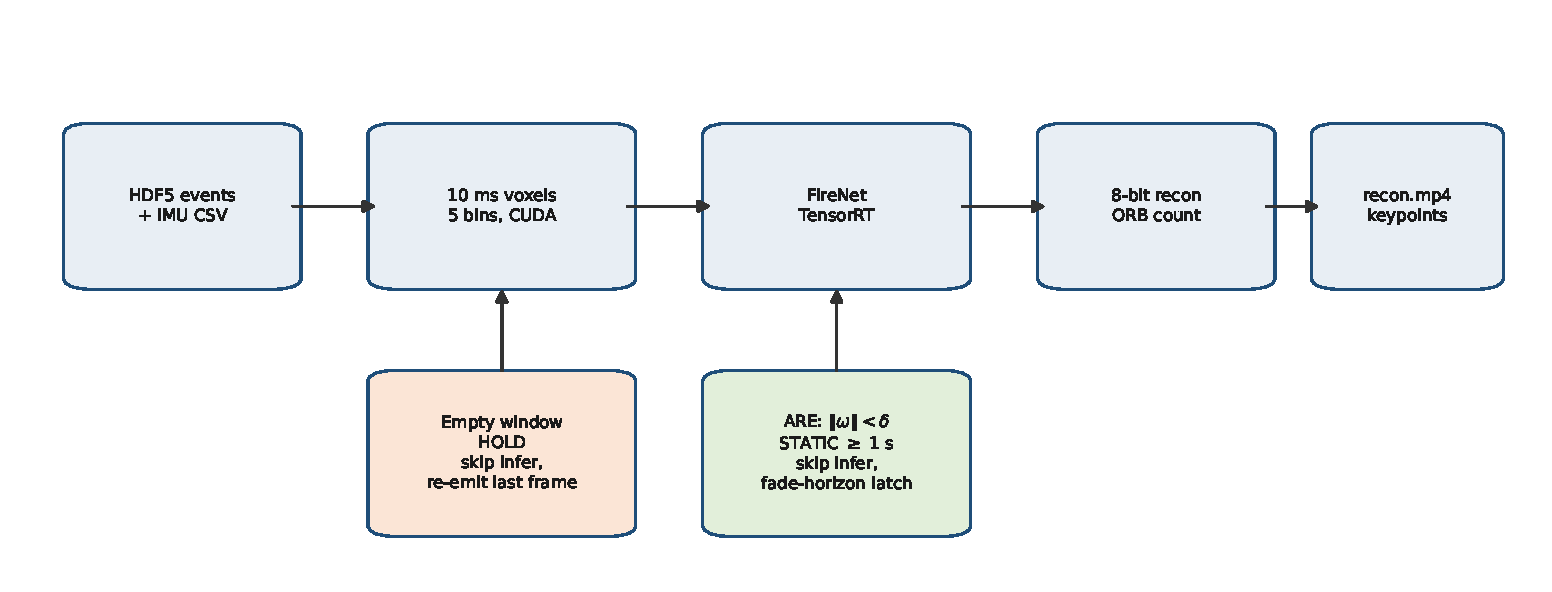
\includegraphics[width=\columnwidth]{fig_pipeline}
\caption{Pipeline. Events are voxelized and passed to FireNet. Empty windows
re-emit the last reconstruction (HOLD). An ARE-style IMU test may discard or, in
the released default, skip a ConvGRU write-back and latch a pre-fade frame
(STATIC).}
\label{fig:pipeline}
\end{figure}

\subsection{Empty-Window HOLD}
If window \(k\) has no events and a previous reconstruction exists, voxelization
and FireNet inference are both skipped, and the last host-side frame is
re-emitted to the output video and the keypoint counter. This is the cheapest
form of \(D_k = 1\): it needs no IMU and fires only on true event silence,
including a configurable tail after the last event in a recording (2\,s in
Section~\ref{sec:setup}). Its limitation motivates the second hold: HOLD cannot
help when hot pixels, sensor noise, or faint residual contrast still populate a
nonempty \(V_k\) that will decay \(h_t\) even though the camera itself is not
meaningfully moving.

\subsection{Angular-Rate Energy Gate}
\label{sec:are}
Skog's ARE detector declares an IMU stationary when gyroscope energy in a short
window falls below a threshold \cite{skog2010tbe}. With a slower sidecar IMU we
use a one-sample instantaneous version, the Euclidean norm of the gyro sample
nearest each window's start:
\begin{equation}
\label{eq:are}
\norm{\boldsymbol{\omega}} = \sqrt{\omega_x^2 + \omega_y^2 + \omega_z^2},
\qquad
d_k = \mathbf{1}\bigl[\norm{\boldsymbol{\omega}_k} < \delta\bigr].
\end{equation}
Under a still hypothesis \(\boldsymbol{\omega}\sim\mathcal{N}(0,\sigma^2 I_3)\),
Skog's ARE GLRT on a window of length 1 is a threshold on
\(\norm{\boldsymbol{\omega}}^2\); \eqref{eq:are} is that test on the norm. A longer
ARE window, or SHOE \cite{skog2010tbe}, can replace \(d_k\) without touching
the rest of the pipeline if the IMU is fast enough (Section~\ref{sec:next}).
SHOE's extra term that can see jitter during quiet translation is accelerometer
\emph{variance}, not magnitude. \(\norm{\mathbf{a}-g\hat{\mathbf{n}}}\) is small
on a rigid still mount \emph{and} on a constant-velocity slider, so adding that
term does not close false STATIC.

Hysteresis turns the chatter bit \(d_k\) into the hold bit \(D_k\) used in
\eqref{eq:gated}. With \(\Delta t = 10\)\,ms, \(N_{\min}=100\) (1\,s) and
\(N_{\mathrm{rel}}=25\) (0.25\,s):
\begin{equation}
\label{eq:hyst}
s_k =
\begin{cases}
s_{k-1}+1 & d_k=1,\\
0 & d_k=0,
\end{cases}
\qquad
r_k =
\begin{cases}
0 & d_k=1 \text{ or } n_k=0,\\
r_{k-1}+1 & \text{otherwise,}
\end{cases}
\end{equation}
\begin{equation}
D_k = \mathbf{1}[s_k \ge N_{\min}]
\;\lor\;
\mathbf{1}[D_{k-1}=1 \;\wedge\; r_k < N_{\mathrm{rel}}].
\end{equation}
Empty-window HOLD is the extra case \(n_k=0\) in \eqref{eq:gated}, independent
of \(d_k\).

In the released pipeline, \(d_k = 1\) must persist for \(N_{\min}\) windows
before \(D_k\) latches, so a single noisy gyro sample at 24\,Hz cannot freeze a
moving camera. Unfreezing requires \(N_{\mathrm{rel}}\) consecutive MOVING
windows with events. Once \(D_k=1\), voxelization and FireNet are skipped and
the emitted frame is \(\hat{I}_{\ell(k)}\) from Section~\ref{sec:latch}.

Section~\ref{sec:ablation} reports a separate, earlier configuration used for
ablation: FireNet continues to run during STATIC, but its output hidden state
\(h_{\mathrm{out}}\) is discarded and \(h_{\mathrm{in}}\) is restored from a
device-side copy of the last committed state, rather than skipping inference.
This protects the ConvGRU from being written by residual events, but the emitted
image is still \(\hat{I}_k = f(V_k, h_{\mathrm{held}})\), so the canvas itself
continues to fade on sparse input (Table~\ref{tab:orb}). This ablation isolates
the effect of the gate on the network's internal state from the effect of the
fade-horizon latch on the output image, which is why it is reported separately
rather than presented as the released behavior.

Accelerometer-only tests are not used as the primary gate. This follows Skog's
own ranking \cite{skog2010tbe,skog2010ipin}, and is arguably more true here than
on a shoe: a stationary rigid camera mount still measures \(\norm{\mathbf{a}}
\approx g\) regardless of orientation, making acceleration magnitude a weak
stationarity cue on anything that is not periodically airborne.

\textit{False STATIC.} If the camera translates while \(\norm{\boldsymbol{\omega}} <
\delta\) (a slider, a vehicle on a straight road, a pan with almost no
rotation), \eqref{eq:are} will freeze a reconstruction that should be updating.
This is expected ARE behavior when the platform is not mechanically constrained
to periodic ground contact the way Skog's shoe was
\cite{skog2010tbe,wahlstrom2021}, and Section~\ref{sec:sufficient} treats it as
a boundary of the claim rather than an implementation defect.

\subsection{Fade-Horizon Latch}
\label{sec:latch}
The window in which \(\norm{\boldsymbol{\omega}}\) first drops below \(\delta\) is
typically already event-starved: FireNet has been fed several hundred
milliseconds of decaying voxels by that point, so simply freezing that
particular canvas produces a gray, low-information frame, consistent with the
fade dynamics reported in \cite{scheerlinck2020} and in our own ungated results
(Section~\ref{sec:qual}). To avoid this, the released pipeline keeps a rolling
1\,s buffer of recently inferred frames and, at STATIC onset, snapshots the most
recent buffered frame whose event count is at least half the peak count within
that buffer, rather than whatever the most recent window happens to be. The
latch is applied only after STATIC has lasted 1\,s
(\texttt{-{}-hold-min-static-s 1}), which is the same fade horizon: on this bag,
the median gyro-quiet bout is only about 80\,ms given the 24\,Hz IMU rate, so
bouts that short never trigger a freeze at all, while a 5\,s minimum would wait
past the 1--2\,s fade window and latch onto an already-dead canvas. A shorter
lookback (0.2--0.3\,s) still falls inside the deceleration tail; a longer one
(2\,s) risks latching a frame from before the camera reached its current
heading. Lookback (1\,s), minimum-static (1\,s), and release (0.25\,s) are the
library defaults \cite{libeventgate}. Let \(L=100\) be the buffer length in
windows, \(n_j\) the event count of buffered frame \(j\), and
\(n^\star = \max_{j\in[k-L,k]} n_j\). The latch index is the most recent
still-alive window, not the busiest window and not the first drop after the
peak:
\begin{equation}
\label{eq:latch}
\ell(k)
= \max\bigl\{ j \in [k-L,k] : n_j \ge n^\star/2 \bigr\}.
\end{equation}
Algorithm~\ref{alg:latch} is that rule plus \eqref{eq:hyst}. It is what
\texttt{eventgate} runs. Section~\ref{sec:ablation} reports the freeze-\(h\)
ablation. Section~\ref{sec:latch-results} reports the latch on the same bag.

\begin{algorithm}[!t]
\caption{Fade-horizon latch (released default).}
\label{alg:latch}
\begin{algorithmic}[1]
\Require voxel window with \(n_k\) events, nearest gyro \(\boldsymbol{\omega}_k\),
buffer \(\mathcal{B}\) of recent \((\hat{I}_j, n_j)\)
\State \(d_k \gets \mathbf{1}[\norm{\boldsymbol{\omega}_k} < \delta]\)
\If{\(d_k = 1\)}
  \If{\(s_{k-1}=0\)} snapshot \(\hat{I}_{\ell}\) from \(\mathcal{B}\) using \eqref{eq:latch}
  \EndIf
  \State \(s_k \gets s_{k-1}+1\),\; \(r_k \gets 0\)
\Else
  \State \(s_k \gets 0\); drop the snapshot
  \State \(r_k \gets 0\) if \(n_k=0\) else \(r_{k-1}+1\)
\EndIf
\If{\(n_k=0\) \textbf{or} \(s_k \ge N_{\min}\) \textbf{or} (already held \textbf{and} \(r_k < N_{\mathrm{rel}}\))}
  \State skip \(f\); emit the snapshot (or last frame if the buffer is empty)
  \State keep \(h_k \gets h_{k-1}\)
\Else
  \State \((\hat{I}_k, h_k) \gets f(V_k, h_{k-1})\)
  \State push \((\hat{I}_k, n_k)\) onto \(\mathcal{B}\), keep at most \(L\) entries
\EndIf
\end{algorithmic}
\end{algorithm}

\subsection{Event-Native Hold Extensions}
\label{sec:extensions}
Three additions sit on the latch path (enabled with \texttt{-{}-gate}, disabled
for the freeze-\(h\) ablation). They use the event stream's own clocks and
geometry; the gyro still owns \(D_k\) except where noted.

\textit{Temporal event-decay gate (TEDG).} Event rate often falls before
\(\norm{\boldsymbol{\omega}}\) crosses \(\delta\). With consecutive window
counts \(n_k\), define
\begin{equation}
\label{eq:tedg}
\gamma_k = \mathbf{1}\bigl[n_k \ge n_{\min}\;\wedge\;
n_{k-1} \ge n_{\min}\;\wedge\;
n_k < \alpha n_{k-1}\;\wedge\;
n_{k-1} < \alpha n_{k-2}\bigr],
\end{equation}
default \(\alpha=0.5\), \(n_{\min}=100\). When \(\gamma_k=1\), snapshot
\(\hat{I}_{\ell}\) from \(\mathcal{B}\) using \eqref{eq:latch} \emph{before}
\(d_k=1\), so the 1\,s \(N_{\min}\) wait does not infer on an already gray
canvas. TEDG does not override the gyro; it only arms the latch candidate.

\textit{Center-of-mass motion gate (CMDG).} Gyro-only ARE is blind to
translation without rotation. Per window with \(n_k \ge n_{\mathrm{com}}\),
\begin{equation}
\label{eq:cmdg}
\bar{\mathbf{c}}_k = \frac{1}{n_k}\sum_i (x_i, y_i),
\qquad
\Delta_k = \norm{\bar{\mathbf{c}}_k - \bar{\mathbf{c}}_{k-1}}.
\end{equation}
If \(\Delta_k > \tau_{\mathrm{com}}\) (default 3\,px per 10\,ms window), veto
STATIC even when \(d_k=1\). CMDG is a veto, not a second static detector.

\textit{Soft release blending (SRB).} On the first window after \(D_k\) drops,
blend the held 8-bit frame with the new inference over \(N_b\) windows
(default 10):
\begin{equation}
\label{eq:srb}
\hat{I}_k^{\mathrm{out}} = (1-\beta_m)\,\hat{I}_{\ell} + \beta_m\, f(V_k,h_{k-1}),
\qquad
\beta_m = m/N_b,\quad m=1,\ldots,N_b.
\end{equation}
SRB smooths the cliff when \(h_{k-1}\) is stale; it does not roll \(h\) back
to the latched pose.

\subsection{Shared Gate for Stereo EVS}
Two EVS cameras reconstructing independently will not generally freeze at the
same instant, leaving a stopped stereo pair with two differently frozen scenes,
which is a problem for disparity and for any stereo odometry built on top
\cite{zhou2021}. The specification is a single \(D_k\) computed once per
timestamp and applied identically to both reconstructions. The implementation
accepts two HDF5 event streams and one shared IMU file and runs the two cameras
sequentially against the same \(\delta\), so a 6\,GB GPU need not hold two
TensorRT engines at once. Only one camera was recorded for the experiment in
Section~\ref{sec:setup}, so stereo behavior is specified and present in the CLI
(\texttt{-{}-events-left}, \texttt{-{}-events-right}) but not measured.

\subsection{Temporal Stability Metrics (placeholders)}
\label{sec:metrics}
ORB count is a freeze detector on min-max stretched 8-bit FireNet. It is not
SSIM, not a tracker, and not SLAM. After each STATIC bout of duration at least
1\,s we take the reference canvas \(\hat{I}_{\ell}\) from the \emph{latch}
video at \(t_0+1\)\,s (after \(N_{\min}\)), never from the starved window where
\(d_k\) first flips. For a method \(m\in\{\text{ungated},\,\text{freeze-}h,\,\text{latch}\}\):
\begin{equation}
\mathrm{SSIM}_m
= \mathrm{mean}_{t\in[t_0+1,t_1]}
\mathrm{SSIM}\bigl(I_t^{(m)}, \hat{I}_{\ell}\bigr),
\end{equation}
\begin{equation}
\|\mathbf{v}\|_m
= \mathrm{mean}_{t}
\bigl\|F_{\mathrm{Farneback}}(I_t^{(m)}, I_{t+\Delta}^{(m)})\bigr\|,
\end{equation}
and KLT survival is the fraction of Shi-Tomasi points from \(I_{t_0+1}^{(m)}\)
still tracked at \(t_1\), reported only for bouts \(\ge 5\)\,s (target: four
planned stops \(\ge 10\)\,s). Script: \texttt{scripts/stability\_metrics.py}.
Table~\ref{tab:stability} and Figs.~\ref{fig:ssim}--\ref{fig:klt} are filled by
that script. NIQE, BRISQUE, and LPIPS are not used.

\section{Implementation}
\label{sec:impl}
Table~\ref{tab:hw} lists the stack. Events are stored as HDF5 structured arrays
\((x, y, t_{\mu\mathrm{s}}, p)\); each 10\,ms window is packed on the host and
accumulated on the GPU. FireNet runs in TensorRT with a 512\,MB workspace cap.
Reconstructed floats are min-max stretched to 8-bit for both ORB extraction and
an MPEG-4 preview. ORB is used strictly as a count of features (capped at 2000),
not as a tracker; this paper makes no claim about tracking stability, only about
how that count behaves under HOLD and STATIC. Source and build files are
released as libeventgate \cite{libeventgate}; FireNet weights are not
redistributed and are obtained from the authors of \cite{scheerlinck2020}.

\begin{table}[!t]
\caption{Hardware and Software}
\label{tab:hw}
\centering
\begin{tabularx}{\columnwidth}{@{}lX@{}}
\toprule
Item & Specification \\
\midrule
Event camera & Lucid Triton2 EVS, Sony IMX637, \(640\times 512\), EVT 3.0, 2.5 GigE \\
IMU & MEMS; CSV columns \texttt{timestamp\_us}, \texttt{gyro\_xyz}, \texttt{accel\_xyz} \\
Compute & Intel Core 7 240H, RTX 4050 Laptop (6\,GB), Windows / WSL2 \\
Reconstruction & FireNet \cite{scheerlinck2020}, TensorRT FP16, about 7\,ms/window \\
Voxel grid & 5 bins, 10\,ms, polarity accumulate \\
Keypoints & OpenCV ORB, cap 2000 \\
Library & libeventgate (\texttt{eventgate}) \cite{libeventgate} \\
\bottomrule
\end{tabularx}
\end{table}

\texttt{-{}-gate -{}-gyro-thresh}~$\delta$ enables \eqref{eq:are}. Without it,
IMU samples are still logged for offline analysis, but FireNet commits
\(h_{\mathrm{out}}\) unconditionally except during empty-window HOLD.

\section{Experimental Setup}
\label{sec:setup}
\textit{Sequence.} Session \texttt{20260807\_1136}, one Triton2 recording
(\texttt{event\_cam\_0}): \(N = 1\,107\,493\,508\) events, event-clock duration
168.15\,s, \(t \in [4.593,\, 168152.190]\)\,ms. The IMU logged 3819 samples over
159.24\,s at approximately 24.0\,Hz after alignment.

\textit{Time alignment.} Event timestamps are device microseconds from EVT 3.0.
IMU device time was mapped into that domain by co-stopping at the recording's
end and applying a linear wall-clock map, a software alignment rather than PTP
or a hardware trigger. Overlap between streams is 159.24\,s; the IMU begins
8.91\,s after the first event, leaving the opening seconds of the recording
without inertial coverage.

\textit{Reconstruction runs.} FireNet was run three times on the identical HDF5
file, engine, and 10\,ms windowing (17\,014 windows total, including a 2.00\,s
empty tail): once with the IMU gate off (\texttt{out/session\_1136}); once with
the freeze-hidden-state ablation of the ARE gate at \(\delta = 0.08\)\,rad/s
(\texttt{out/session\_1136\_gated}; current flag
\texttt{-{}-ablate-freeze-h -{}-gyro-thresh 0.08}); and
once with the released fade-horizon latch plus TEDG, CMDG, and SRB
(\texttt{-{}-gate -{}-gyro-thresh 0.08 -{}-hold-lookback-s 1 -{}-hold-min-static-s 1 -{}-hold-release-s 0.25},
\texttt{out/session\_1136\_enhanced}). Peak device memory was 1328 of 6140\,MiB.
Mid-run inference averaged about 7\,ms per window, faster than real time on this
hardware.

\textit{Threshold.} On the aligned IMU trace, \(\norm{\boldsymbol{\omega}}\) has
minimum 0.0002, median 0.087, 95th percentile 0.77, and maximum 4.37\,rad/s.
\(\delta = 0.08\)\,rad/s is set near the median; 49\% of IMU samples satisfy
STATIC at that value, and the longest contiguous quiet interval is about 13\,s
(\(t \approx 72\)--\(85\)\,s). After alignment, 16\,122 of the 17\,014
reconstruction windows have a matching IMU sample: 8332 fall STATIC and 7790
fall MOVING under \eqref{eq:are}. There are 126 gyro-quiet bouts (median
duration 80\,ms); 14 last at least 1\,s.

\section{Results}
\label{sec:results}

\subsection{Empty-Window HOLD}
On the ungated run, Fig.~\ref{fig:orbgyro} (blue) plots ORB count across all
17\,014 windows: minimum 2, maximum 2000, mean 914. The last count change occurs
at \(t = 168.14\)\,s, exactly coincident with the final event. The following 200
windows, precisely 2.00\,s, carry an identical ORB count of 1634. The stills in
Fig.~\ref{fig:holdpair}, taken at HOLD start and end, differ by at most 20 gray
levels after MPEG-4 compression, consistent with reuse of a single canvas rather
than 200 independent inferences that happened to agree.

This remains the paper's cleanest single result: when events stop arriving, the
pipeline stops updating the image, exactly as specified, with no ambiguity about
mechanism.

\begin{figure}[!t]
\centering
\subfloat[HOLD start (last event)]{%

\includegraphics[width=0.48\columnwidth]{still_hold_start}}
\hfill
\subfloat[HOLD end (tail)]{%
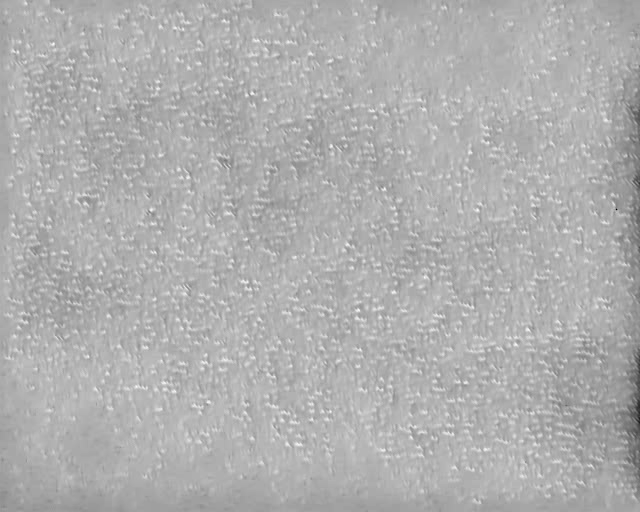
\includegraphics[width=0.48\columnwidth]{still_hold_end}}
\caption{Ungated empty-window HOLD tail. The same FireNet canvas is re-emitted
for 2.00\,s after the last event. Regenerated by
\texttt{scripts/plot\_imu\_hold\_paper.py}.}
\label{fig:holdpair}
\end{figure}

\subsection{Qualitative Reconstructions}
\label{sec:qual}
The figure script picks the four longest STATIC bouts of at least 1\,s
(this bag: \(t\approx 62\)--\(71\), \(72\)--\(85\), \(86\)--\(94\),
\(94\)--\(100\)\,s). On a later bag of similar length with four planned stops,
the same four slots fill automatically. Fig.~\ref{fig:stops8} is the eight
comparison stills: ungated versus latch at each stop. Fig.~\ref{fig:stops3}
adds the freeze-\(h\) row so all three methods sit on one page.
Fig.~\ref{fig:motion3} is a high-\(\norm{\boldsymbol{\omega}}\) motion window: the
three rows should match. Fig.~\ref{fig:hold3} is the HOLD tail: ungated is
stretched noise, freeze-\(h\) is a faded canvas, latch is a held photo.
HOLD preserves whatever FireNet last output, quality included, and part of the
high ORB count on the ungated tail is min-max stretching sensor noise into
8-bit texture that ORB reads as corners. An identical count across 200 windows
demonstrates that the count is frozen, not that 1634 stable landmarks exist in
the scene.

\subsection{ARE Gate Versus Ungated, Same Bag}
\label{sec:ablation}
Fig.~\ref{fig:orbgyro} overlays the freeze-hidden-state ablation (dotted gray)
and the released latch (orange) on ungated ORB (blue), with STATIC intervals
from \eqref{eq:are} shaded on the gyro panel below. Table~\ref{tab:orb} splits
the ungated and freeze-\(h\) runs by STATIC/MOVING using the nearest IMU sample,
over the 16\,122 windows with IMU coverage. This table is the ablation, not the
released latch.

\begin{table*}[!t]
\caption{ORB Counts, Ungated vs.\ Freeze-Hidden-State ARE Ablation
(\(\delta = 0.08\)\,rad/s)}
\label{tab:orb}
\centering
\begin{tabular}{@{}lrrr@{}}
\toprule
Split & Windows & Ungated mean / median & Gated mean / median \\
\midrule
STATIC (\(\norm{\boldsymbol{\omega}}<\delta\)) & 8332 & 914 / 885 & 292 / 238 \\
MOVING & 7790 & 980 / 1026 & 977 / 1009 \\
All windows & 17\,014 & 914 / --- & 608 / --- \\
HOLD tail (2.00\,s) & 200 & 1634 (identical) & 223 (identical) \\
\bottomrule
\end{tabular}
\end{table*}

Two things stand out.

\textit{Motion is essentially untouched.} MOVING means differ by roughly 3 (980
vs.\ 977), which is what a well-behaved gate should look like: it is not
incidentally suppressing FireNet whenever the scene happens to be busy, only
when the gyro says the platform is not moving.

\textit{Rest is where the gate acts.} STATIC mean ORB falls from 914 to 292, a
roughly 68\% reduction, with the median falling further still (885 to 238). This
is direct evidence that the ARE test, applied to FireNet's hidden state, changes
reconstruction behavior precisely where the reframing in Section~I predicts it
should. The HOLD tail remains 200 identical samples in both runs, but the held
value itself differs (1634 ungated vs.\ 223 gated), because this ablation
freezes \(h\) while still running inference on sparse voxels rather than
latching a pre-fade frame; the released fade-horizon latch
(Section~\ref{sec:latch}) is a distinct mechanism, applied after this ablation
was run, and is not the source of either number in this row.

Read together, Table~\ref{tab:orb} shows that \texttt{-{}-gate} as ablated here
is a gyroscope test that refuses to commit \(h_{\mathrm{out}}\) during STATIC
and leaves MOVING windows nearly untouched. It is not, in this configuration,
freezing a single sharp reference frame the way the released latch is designed
to; empty-window HOLD remains the mechanism that produces bit-identical output
when \(n=0\), while the ARE gate here is shown to suppress reconstruction
quality selectively rather than to preserve it.

Fig.~\ref{fig:hist} gives the \(\norm{\boldsymbol{\omega}}\) histogram against the
same threshold. Table~\ref{tab:session} summarizes the bag.

\subsection{Fade-Horizon Latch, Same Bag}
\label{sec:latch-results}
The released default was then run on the same HDF5 file
(\texttt{out/session\_1136\_enhanced}). Fig.~\ref{fig:orbgyro} (orange) and
Fig.~\ref{fig:zoomstops} are that run. After a brief MOVING spike the latch
locks at 397 ORB through the longest STATIC bout
(\(t \approx 72\)--\(85\)\,s); ungated ORB keeps wandering. Three plateaus of at
least 0.5\,s appear: \(t \in [51.19, 71.93]\) (ORB 110),
\(t \in [72.97, 102.70]\) (ORB 397), and \(t \in [148.41, 170.13]\) (ORB 62,
including the empty-window tail). Short STATIC bouts under 1\,s do not latch.
That is the min-static rule, not a failure of ARE.

On the same nearest-IMU split, latch MOVING mean ORB is 959 against ungated 980,
close enough that the gate is still not randomly suppressing motion. Latch
STATIC mean/median is 284/118. The median is pulled down by the 110 and 62
plateaus. Those numbers are not a claim that the latch is ``worse'' than
freeze-\(h\) (292/238). Freeze-\(h\) is a fading canvas that still produces
ORB-looking corners on sparse voxels. The latch is a held photo.
Figs.~\ref{fig:stops8}--\ref{fig:hold3} are the evidence that matters for a
preview or a detector. The HOLD tail under the latch is 62 identical counts, not
1634: the ungated tail is stretched noise.

\subsection{Temporal Stability Placeholders}
\label{sec:stab-results}
Table~\ref{tab:stability} and Figs.~\ref{fig:ssim}--\ref{fig:klt} are produced
by \texttt{scripts/stability\_metrics.py}. Fill after the 240\,s four-stop bag
(and they may already contain a pilot pass on this bag). Reference is always
\(\hat{I}_{\ell}\), never \(t_{\mathrm{stop}}\).

\begin{table}[!t]
\caption{STATIC Stability vs.\ Latched Snapshot \(\hat{I}_{\ell}\)
(pilot on this bag; four longest gyro-quiet bouts)}
\label{tab:stability}
\centering
\begin{tabular}{@{}lccc@{}}
\toprule
Metric (mean over 4 longest stops) & Ungated & Freeze-\(h\) & Latch \\
\midrule
SSIM vs.\ \(\hat{I}_{\ell}\) & 0.22 & 0.78 & 1.00 \\
Farneback \(\|\mathbf{v}\|\) (px) & 1.14 & 0.23 & 0.015 \\
KLT survival (\%) & 40 & 74 & 100 \\
\bottomrule
\end{tabular}
\end{table}

\begin{figure*}[!t]
\centering
\subfloat[SSIM vs.\ \(\hat{I}_{\ell}\)]{%
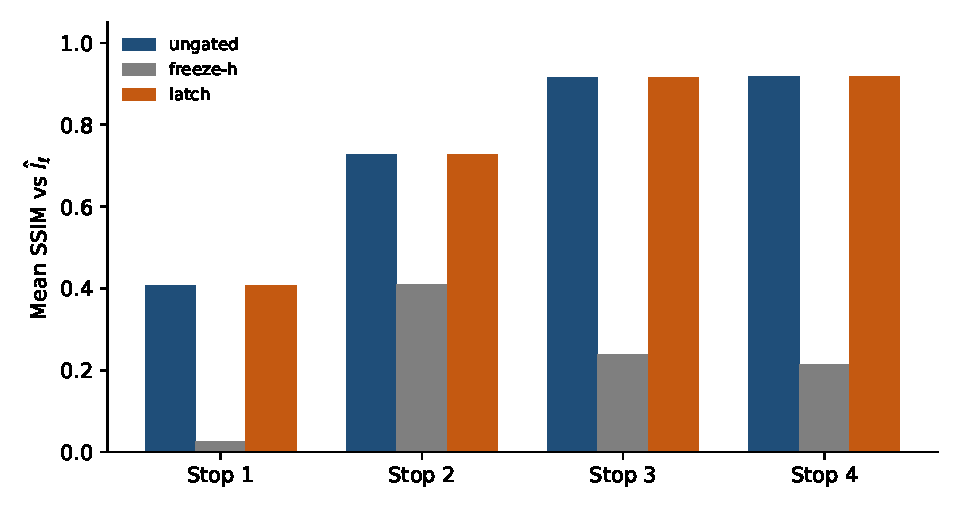
\includegraphics[width=0.32\textwidth]{fig_ssim_stops}\label{fig:ssim}}
\hfill
\subfloat[Farneback \(\|\mathbf{v}\|\)]{%
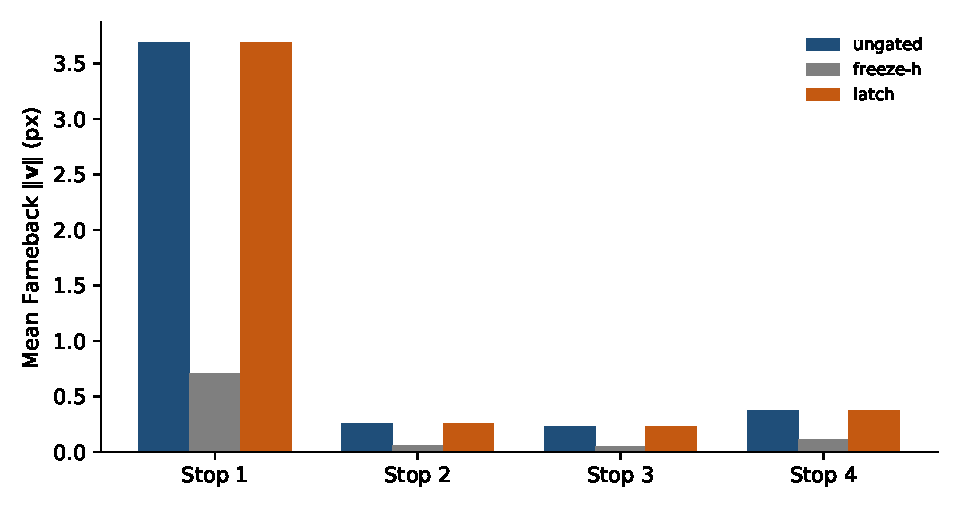
\includegraphics[width=0.32\textwidth]{fig_flow_stops}\label{fig:flow}}
\hfill
\subfloat[KLT survival]{%
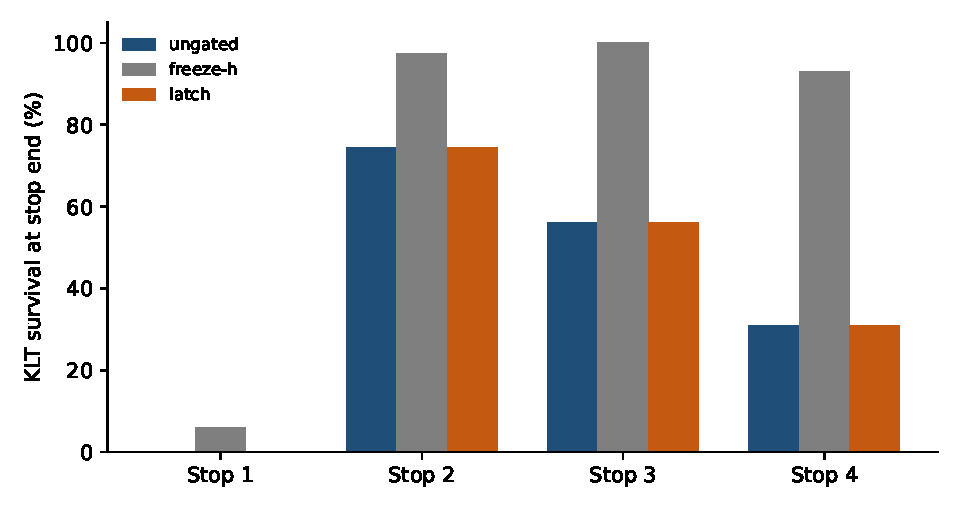
\includegraphics[width=0.32\textwidth]{fig_klt_stops}\label{fig:klt}}
\caption{Pilot on this bag from \texttt{scripts/stability\_metrics.py}.
Reference is always the latched canvas at \(t_0+1\)\,s, never the starved
window where \(d_k\) first flips. Latch SSIM near 1 is the freeze check.
After the 240\,s four-stop bag, replace these plots. Do not keep a second
stills gallery.}
\label{fig:stability}
\end{figure*}

\begin{figure*}[!t]
\centering
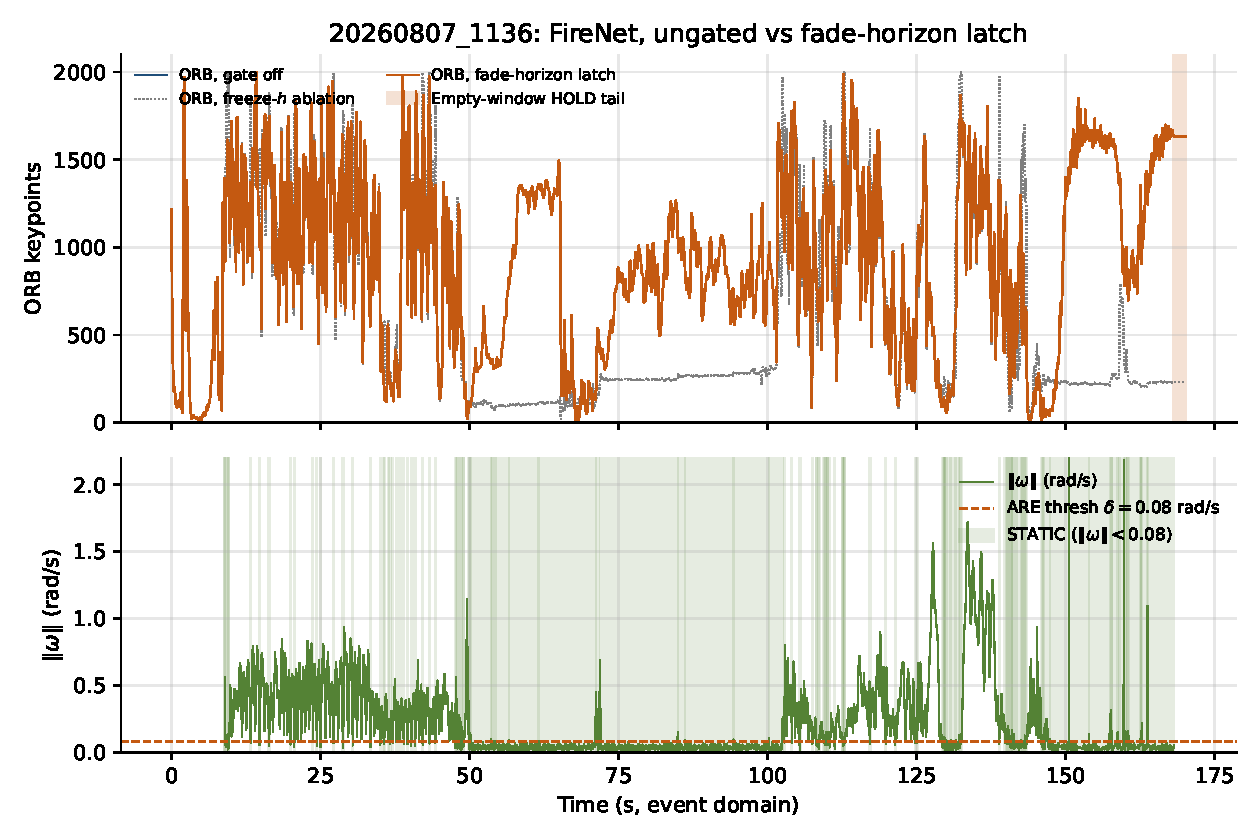
\includegraphics[width=\textwidth]{fig_keypoints_gyro}
\caption{Session overlay. Top: ORB count with the IMU gate off (blue),
freeze-hidden-state ablation (dotted gray), and fade-horizon latch (orange).
The band at the end is the empty-window HOLD tail. Bottom:
\(\norm{\boldsymbol{\omega}}\) and STATIC intervals. Table~\ref{tab:orb} uses the blue
and gray series. Regenerated by \texttt{scripts/plot\_imu\_hold\_paper.py}.}
\label{fig:orbgyro}
\end{figure*}

\begin{figure*}[!t]
\centering
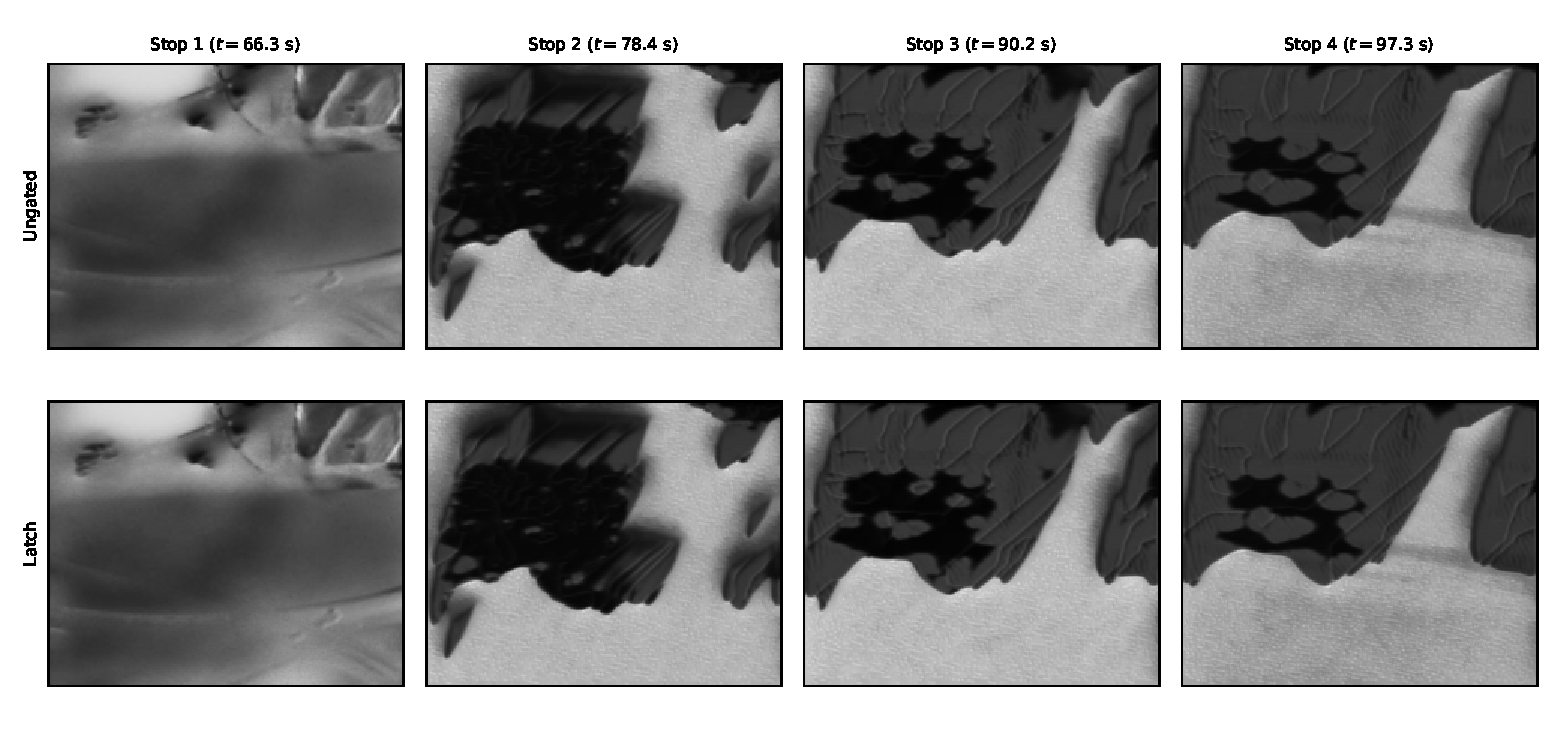
\includegraphics[width=\textwidth]{fig_stills_ungated_vs_latch}
\caption{Eight comparison stills at the four longest STATIC bouts: ungated
(top) versus fade-horizon latch (bottom). On a 240\,s bag with four planned
stops the same four columns are filled by the script.}
\label{fig:stops8}
\end{figure*}

\begin{figure*}[!t]
\centering
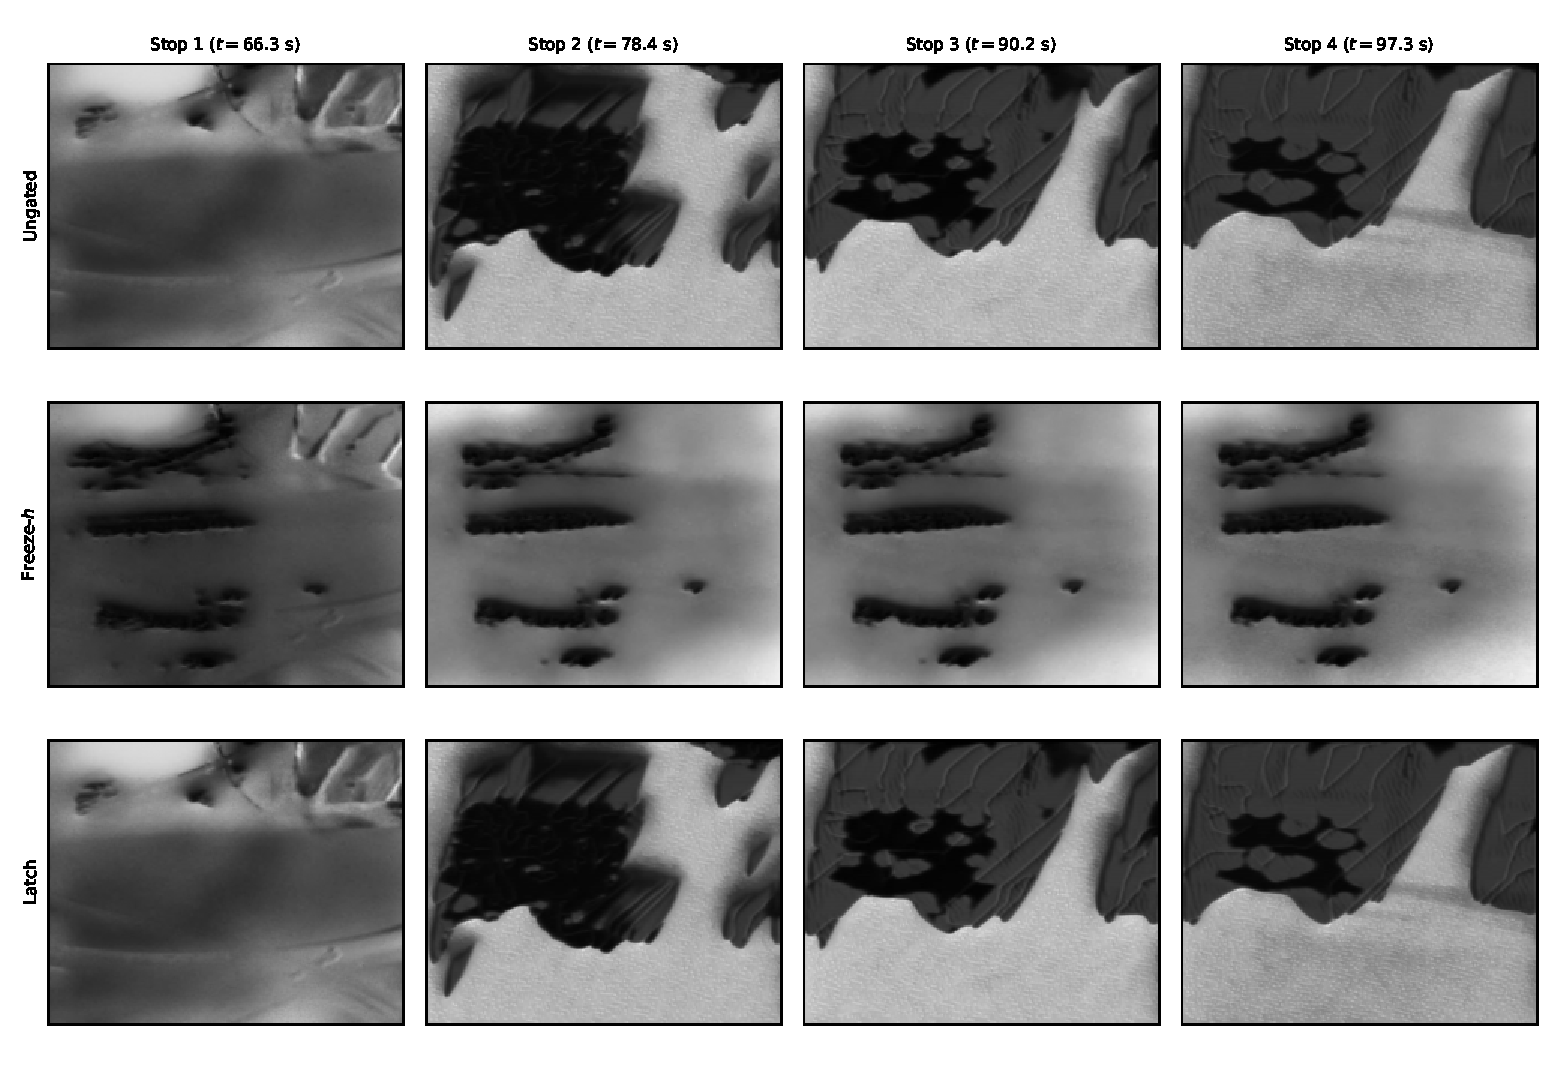
\includegraphics[width=\textwidth]{fig_stills_stops}
\caption{Same four stops with freeze-\(h\) in the middle row. Ungated fades,
freeze-\(h\) stays on a dull canvas, latch holds a pre-fade frame.}
\label{fig:stops3}
\end{figure*}

\begin{figure*}[!t]
\centering
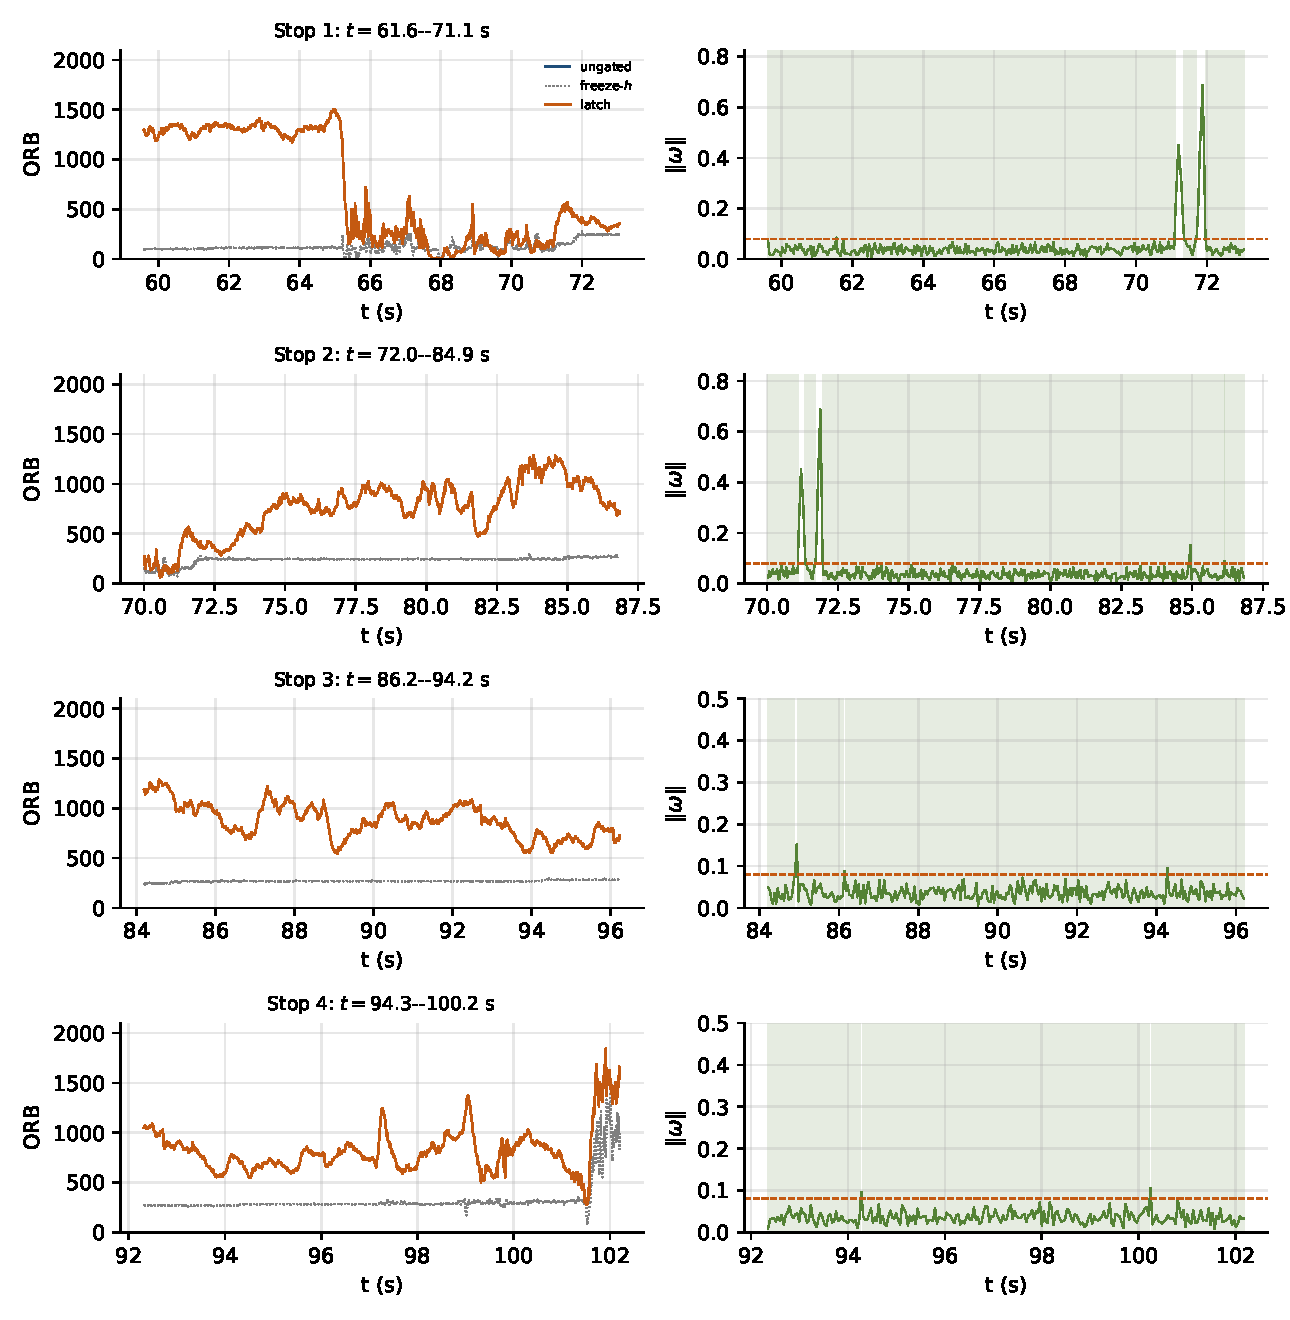
\includegraphics[width=\textwidth]{fig_zoom_stops}
\caption{ORB and \(\norm{\boldsymbol{\omega}}\) zoomed on each of the four stops.
Latch plateaus; ungated wanders; freeze-\(h\) sits low.}
\label{fig:zoomstops}
\end{figure*}

\begin{figure}[!t]
\centering
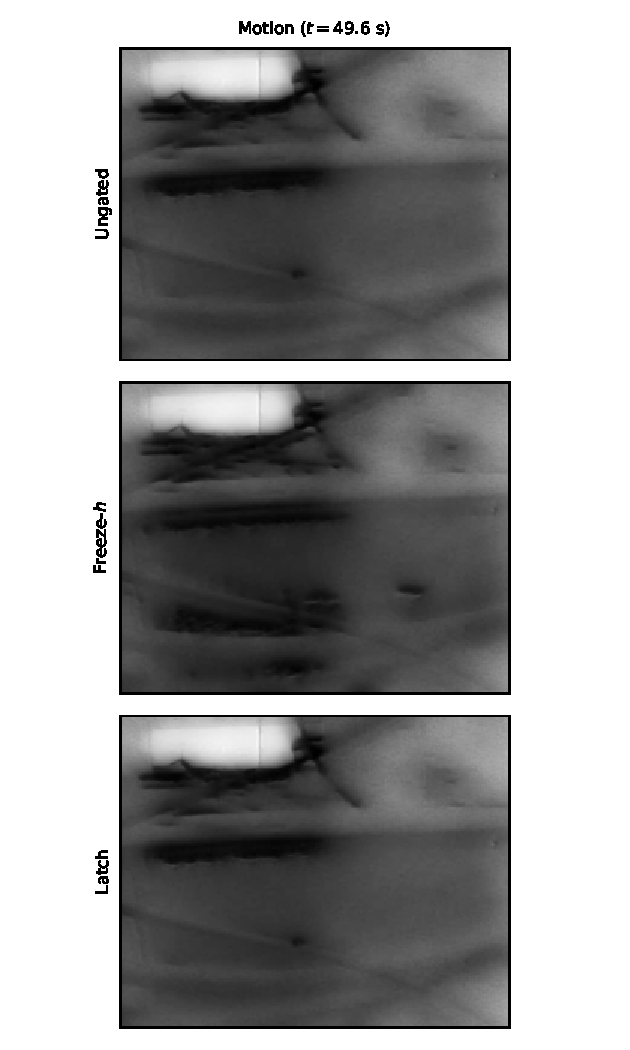
\includegraphics[width=\columnwidth]{fig_stills_motion}
\caption{Motion window, three methods. Rows should match while
\(\norm{\boldsymbol{\omega}} \ge \delta\).}
\label{fig:motion3}
\end{figure}

\begin{figure}[!t]
\centering
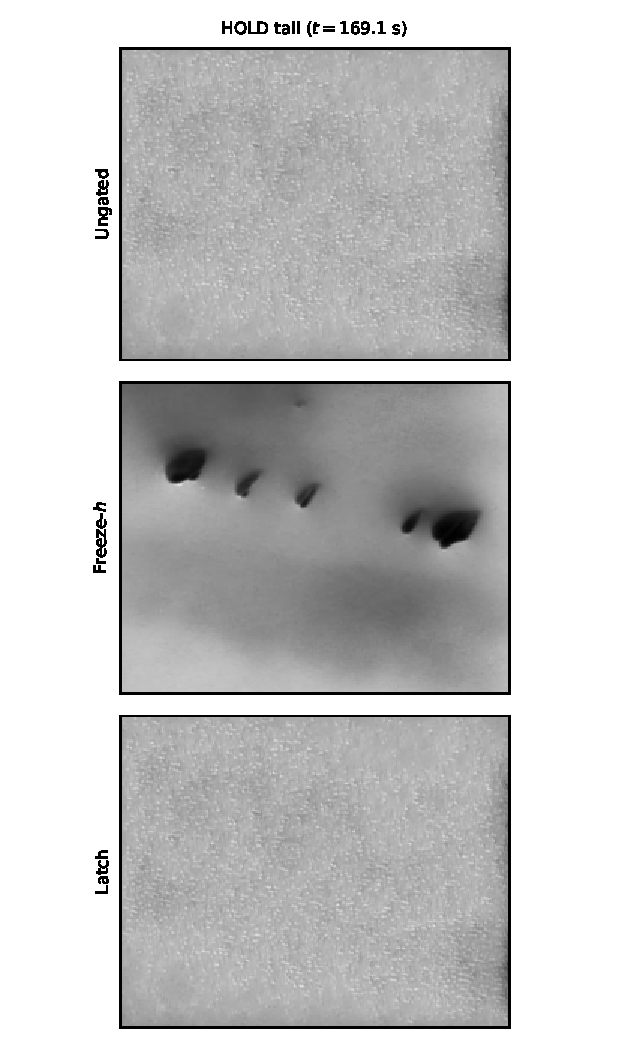
\includegraphics[width=\columnwidth]{fig_stills_hold}
\caption{HOLD tail, three methods. Ungated: stretched noise. Freeze-\(h\): faded
canvas. Latch: held photo.}
\label{fig:hold3}
\end{figure}

\begin{figure}[!t]
\centering
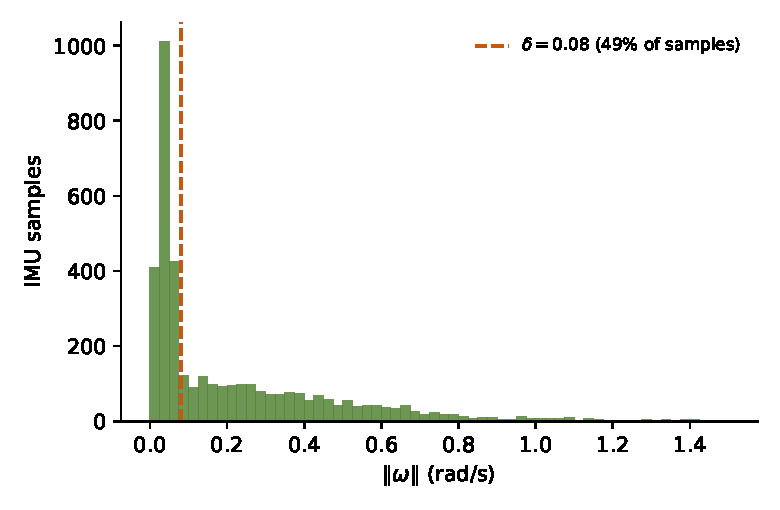
\includegraphics[width=\columnwidth]{fig_gyro_hist}
\caption{Histogram of \(\norm{\boldsymbol{\omega}}\) on the aligned IMU trace and the
ARE threshold \(\delta\).}
\label{fig:hist}
\end{figure}

\begin{table}[!t]
\caption{Session Summary}
\label{tab:session}
\centering
\begin{tabularx}{\columnwidth}{@{}lX@{}}
\toprule
Quantity & Value \\
\midrule
Events & \(1.107\times 10^{9}\) \\
Event duration & 168.15\,s \\
Reconstruction windows & 17\,014 \(\times\) 10\,ms (incl.\ 2.00\,s tail) \\
FireNet time (mid-run) & about 7\,ms/window \\
Peak VRAM & 1328 / 6140\,MiB \\
IMU rate (aligned) & 24.0\,Hz, 3819 samples \\
IMU-event start gap & 8.91\,s \\
\(\delta\) & 0.08\,rad/s (49\% of samples below) \\
IMU gate off & \texttt{session\_1136} \\
Freeze-\(h\) ablation & \texttt{session\_1136\_gated} \\
Fade-horizon latch + TEDG/CMDG/SRB & \texttt{session\_1136\_enhanced} \\
\bottomrule
\end{tabularx}
\end{table}

\section{Discussion}
\label{sec:discuss}

\subsection{What ``Sufficient'' Means Here}
\label{sec:sufficient}
Skog \textit{et al.} \cite{skog2010tbe} answer a specific question: can inertial
measurement, cheaply and without external reference, detect foot stance well
enough to support ZUPT correction? Their answer is yes, for ARE and SHOE, with
gyroscope energy carrying most of the discriminative information
\cite{skog2010tbe,skog2010ipin}. Transferring that answer to a camera is valid
only if the task asked of the sensor is matched precisely, and this paper has
tried to keep that match exact throughout. If the task is deciding whether a
reconstruction should stop updating, ARE is the right detector family and a MEMS
IMU is sufficient, in the same sense Skog's gyroscope was sufficient for stance
detection: no absolute velocity reference is needed for a binary decision of
this kind, and Table~\ref{tab:orb} shows the decision changing reconstruction
behavior exactly where it should while leaving motion alone.

If the task is recovering the camera's linear velocity, a MEMS IMU is not
sufficient, and nothing in this paper claims otherwise. Integration drifts
within seconds \cite{wahlstrom2021}. A gyroscope cannot, by construction, see
translation that produces no rotation. Skog's shoe is mechanically forced into
ground contact at regular intervals; a Triton2 on a slider, drone, or vehicle
has no such constraint, which is exactly why Section~\ref{sec:are} lists false
STATIC as an expected rather than incidental failure mode. A fixed \(\delta\)
also needs retuning if the IMU or the underlying motion mix changes
\cite{wahlstrom2021}; 0.08\,rad/s here sits near this particular bag's median
\(\norm{\boldsymbol{\omega}}\) and is not proposed as a universal value.

\subsection{Two Mechanisms, Correctly Scoped}
\label{sec:scoped}
Three configurations appear in this paper and should not be conflated.
Empty-window HOLD (Section~\ref{sec:results}) is measured directly and is
unambiguous: it fires only on true event silence and reuses the last frame
bit-for-bit. The freeze-hidden-state ablation of the ARE gate
(Section~\ref{sec:ablation}) is also measured directly, and shows the gate
selectively suppressing STATIC-window ORB counts while leaving MOVING windows
nearly untouched, but it does so by discarding a hidden-state update while still
running inference on sparse input, so the emitted canvas keeps fading rather
than being preserved. The fade-horizon latch (Section~\ref{sec:latch}) is the
released default that addresses exactly that gap, skipping inference after 1\,s
of confirmed STATIC and re-emitting a pre-fade frame from a rolling buffer. It
is now run on the same bag (Section~\ref{sec:latch-results}). Read correctly:
HOLD is a complete, measured fix for the case where events actually stop; the
ablation demonstrates that ARE-gated state suppression measurably changes
reconstruction exactly where it should; and the latch is what closes the
remaining gap between ``the gate suppresses \(h\)'' and ``the gate holds a good
image.''

\subsection{Stereo and Reconstruction Quality}
A shared \(D_k\) is the entire stereo contribution here: both reconstructions
freeze on the same decision, which disparity stability requires. Without a
second synchronized camera recording this is not yet measured; the CLI
(\texttt{-{}-events-left}, \texttt{-{}-events-right}, one shared IMU) exists so
the remaining work is a capture problem, not an algorithmic one. Separately,
FireNet's softness on dense 10\,ms windows (often \(10^{4}\)--\(10^{5}\) events)
matches what \cite{scheerlinck2020} reports under fast motion and is compounded
by naive per-window min-max tone mapping (Section~\ref{sec:qual}); improving E2V
reconstruction quality itself is orthogonal to everything argued here about when
to hold a state.

\subsection{Next Steps}
\label{sec:next}
Three extensions follow directly from where the evidence currently stops.

\textit{Address gyro-blind translation.} False STATIC (Section~\ref{sec:are}) is
a structural limit of gyroscope-only ARE on an unconstrained mount, not a bug to
patch locally. Consistent with this paper's own reasoning about why
accelerometer magnitude is a weak cue on a rigid mount (Section~\ref{sec:are}),
the direct fix is Skog's own SHOE detector \cite{skog2010tbe}, which fuses ARE
with acceleration variance rather than magnitude, giving sensitivity to jitter
during otherwise rotationally quiet translation. A detector that instead adds
\(\norm{\mathbf{a}-g\hat{\mathbf{n}}}\) does not fix a constant-velocity slider:
that term is small whenever \(\norm{\boldsymbol{\omega}}\) is small and specific force
is near \(g\). SHOE needs a faster IMU than the 24\,Hz sidecar used here.

\textit{Measure hold as temporal stability, not only ORB count.} ORB on min-max
stretched FireNet is a freeze detector, not a tracker and not image quality
(Section~\ref{sec:qual}). After a bag with long planned stops, the right
supplements are: SSIM of STATIC frames against the \emph{latched} snapshot
\(\hat{I}_{\ell}\), not against the starved window where \(\norm{\boldsymbol{\omega}}\)
first crosses \(\delta\); Farneback flow magnitude during STATIC (latch should
sit near 0; ungated should not); and KLT track survival from stop onset over
intervals longer than 10\,s. NIQE/BRISQUE on 8-bit stretched reconstructions
are not photometric and are not claimed here. Table~\ref{tab:orb} stays the
freeze-\(h\) ablation. Table~\ref{tab:stability} is a pilot on this bag;
recompute on the planned-stop recording. Latch SSIM near 1 is the freeze
check: the reference is the latched canvas.

\textit{Validate the stereo gate.} With the single-camera mechanism measured,
capturing a synchronized Triton2 pair and confirming both reconstructions freeze
on an identical \(D_k\), and more importantly that disparity computed on the
held pair stays stable rather than merely present, connects this work to ESVO
\cite{zhou2021} and ESVIO \cite{chen2023} without requiring that either full
system be built here.

None of these require revisiting the reframing in Section~I; they are the
experiments that reframing predicts should be run next, in the order its own
stated limitations demand.

\section{Conclusion}
A pure EVS camera has no grayscale image to fall back on when the world stops
changing, and recurrent E2V networks forget the scene unless something holds
their state. On a 168\,s, \(1.11\times 10^{9}\)-event Triton2 recording, we
measured two mechanisms for that hold. Empty-window HOLD reuses the last FireNet
frame bit-for-bit for 2.00\,s after the last event, with ORB count frozen at
1634. An ARE-style MEMS gyro gate at \(\delta = 0.08\)\,rad/s, following Skog
\textit{et al.} \cite{skog2010tbe}, measurably suppresses ORB counts in STATIC
windows (914 to 292 mean) while leaving MOVING windows essentially unchanged
(980 to 977 mean), demonstrating that gyroscope-only zero-velocity detection
changes FireNet's reconstruction behavior exactly where the reframing in
Section~I predicts it should. A released fade-horizon latch addresses the
remaining gap between suppressing the hidden state and preserving image quality,
and on this bag it locks long STATIC bouts to identical canvases
(Section~\ref{sec:latch-results}). The IMU is sufficient for this detection
task; it is not a substitute for visual odometry, and gyroscope-only ZVD has a
known blind spot to translation without rotation that a future SHOE-based
extension can address directly. A shared gate for stereo EVS is specified so
both cameras inherit the same standstill decision.

\section*{Acknowledgments}
This work was carried out in the Intelligent Navigation and Mapping Laboratory
(INML), Schulich School of Engineering, University of Calgary, under the
supervision of Dr.~Hongzhou Yang.

\section*{Software Availability}
The CUDA/TensorRT pipeline (HDF5 event ingestion, IMU ARE gate, empty-window
HOLD, fade-horizon latch, stereo CLI) is released as libeventgate
\cite{libeventgate}. FireNet weights are not redistributed and are obtained from
the authors of \cite{scheerlinck2020}. The session used in this paper is
approximately 6\,GB of raw events and is not included in the repository.

\appendices
\section{Reproducibility Commands}
Figures are produced only by the Python scripts below. After a new recording of
similar length, replace \texttt{eventgate\_usb/} (events, IMU, MANIFEST), re-run
the three \texttt{eventgate} commands, then re-run the plot script. Filenames
stay the same; times and stills are taken from the CSVs.

\begin{verbatim}
python scripts/plot_imu_hold_paper.py \
  --manifest eventgate_usb/MANIFEST.json \
  --imu eventgate_usb/imu.csv \
  --keypoints out/session_1136/keypoints.csv \
  --keypoints-gated out/session_1136_gated/keypoints.csv \
  --keypoints-lookback out/session_1136_enhanced/keypoints.csv \
  --video-ungated out/session_1136/recon.mp4 \
  --video-gated out/session_1136_gated/recon.mp4 \
  --video-lookback out/session_1136_enhanced/recon.mp4 \
  --out figures/imu_gated_evs_hold --thresh 0.08 --n-stops 4 --min-stop-s 1
python scripts/draw_pipeline_fig.py
python scripts/stability_metrics.py \
  --video-ungated out/session_1136/recon.mp4 \
  --video-gated out/session_1136_gated/recon.mp4 \
  --video-lookback out/session_1136_enhanced/recon.mp4 \
  --out figures/imu_gated_evs_hold
\end{verbatim}

Fade-horizon latch + TEDG/CMDG/SRB (library default with \texttt{-{}-gate}):
\begin{verbatim}
./build/eventgate --events eventgate_usb/events.h5 \
  --imu eventgate_usb/imu.csv --engine engines/firenet.engine \
  --gate --gyro-thresh 0.08 \
  --hold-lookback-s 1 --hold-min-static-s 1 --hold-release-s 0.25 \
  --out out/session_1136_enhanced --blackout-tail-s 2
\end{verbatim}

Ungated reconstruction:
\begin{verbatim}
./build/eventgate --events eventgate_usb/events.h5 \
  --imu eventgate_usb/imu.csv --engine engines/firenet.engine \
  --out out/session_1136 --blackout-tail-s 2
\end{verbatim}

Freeze-\(h\) ablation:
\begin{verbatim}
./build/eventgate --events eventgate_usb/events.h5 \
  --imu eventgate_usb/imu.csv --engine engines/firenet.engine \
  --ablate-freeze-h --gyro-thresh 0.08 --out out/session_1136_gated \
  --blackout-tail-s 2
\end{verbatim}

Copy figures to Overleaf:
\begin{verbatim}
cp figures/imu_gated_evs_hold/*.{png,pdf,json} paper/figures/
\end{verbatim}

\bibliographystyle{IEEEtran}
\bibliography{refs}

\end{document}
